%%%%%%%%%%%%%%%%%%%%%%%%%%%%%%%%%%%%%%%%%%%%%%%%%%%%%%%%%%%%%%%%%%%%%%%
%% template for II2202 report
%% original 2015.11.24
%% revised  2018.08.26
%%%%%%%%%%%%%%%%%%%%%%%%%%%%%%%%%%%%%%%%%%%%%%%%%%%%%%%%%%%%%%%%%%%%%%%
%

\title{Supporting personnel in warehouses with an inertial measurement unit}
\author{
        \textsc{Adrian Ackva}
            \qquad
        \textsc{Gabor Finta}
        \mbox{}\\
        \normalsize
            \texttt{ackva@kth.se}
        \textbar{}
            \texttt{finta}
        \normalsize
            \texttt{@kth.se}
}
\date{\today}

\documentclass[12pt,twoside, hidelinks]{article}

\usepackage[paper=a4paper,dvips,top=1.5cm,left=1.5cm,right=1.5cm,
    foot=1cm,bottom=1.5cm]{geometry}


%\usepackage[T1]{fontenc}
%%\usepackage{pslatex}
\renewcommand{\rmdefault}{ptm} 
\usepackage{mathptmx}
\usepackage[scaled=.90]{helvet}
\usepackage{courier}
%
\usepackage{bookmark}

\usepackage{fancyhdr}
\pagestyle{fancy}

%%----------------------------------------------------------------------------
%%   pcap2tex stuff
%%----------------------------------------------------------------------------
 \usepackage[dvipsnames*,svgnames]{xcolor} %% For extended colors
 \usepackage{tikz}
 \usetikzlibrary{arrows,decorations.pathmorphing,backgrounds,fit,positioning,calc,shapes}

%% \usepackage{pgfmath}	% --math engine
%%----------------------------------------------------------------------------
%% \usepackage[latin1]{inputenc}
\usepackage[utf8]{inputenc} % inputenc allows the user to input accented characters directly from the keyboard
\usepackage[swedish,english]{babel}
%% \usepackage{rotating}		 %% For text rotating
\usepackage{array}			 %% For table wrapping
\usepackage{graphicx}	                 %% Support for images
\usepackage{float}			 %% Suppor for more flexible floating box positioning
\usepackage{color}                       %% Support for colour 
\usepackage{mdwlist}
%% \usepackage{setspace}                 %% For fine-grained control over line spacing
%% \usepackage{listings}		 %% For source code listing
%% \usepackage{bytefield}                %% For packet drawings
\usepackage{tabularx}		         %% For simple table stretching
%%\usepackage{multirow}	                 %% Support for multirow colums in tables
\usepackage{dcolumn}	                 %% Support for decimal point alignment in tables
\usepackage{url}	                 %% Support for breaking URLs
\usepackage[perpage,para,symbol]{footmisc} %% use symbols to ``number'' footnotes and reset which symbol is used first on each page

%% \usepackage{pygmentize}           %% required to use minted -- see python-pygments - Pygments is a Syntax Highlighting Package written in Python
%% \usepackage{minted}		     %% For source code highlighting

%% \usepackage{hyperref}		
\usepackage[all]{hypcap}	 %% Prevents an issue related to hyperref and caption linking
%% setup hyperref to use the darkblue color on links
%% \hypersetup{colorlinks,breaklinks,
%%             linkcolor=darkblue,urlcolor=darkblue,
%%             anchorcolor=darkblue,citecolor=darkblue}

%% Some definitions of used colors
\definecolor{darkblue}{rgb}{0.0,0.0,0.3} %% define a color called darkblue
\definecolor{darkred}{rgb}{0.4,0.0,0.0}
\definecolor{red}{rgb}{0.7,0.0,0.0}
\definecolor{lightgrey}{rgb}{0.8,0.8,0.8} 
\definecolor{grey}{rgb}{0.6,0.6,0.6}
\definecolor{darkgrey}{rgb}{0.4,0.4,0.4}
%% Reduce hyphenation as much as possible
\hyphenpenalty=15000 
\tolerance=1000

%% useful redefinitions to use with tables
\newcommand{\rr}{\raggedright} %% raggedright command redefinition
\newcommand{\rl}{\raggedleft} %% raggedleft command redefinition
\newcommand{\tn}{\tabularnewline} %% tabularnewline command redefinition

%% definition of new command for bytefield package
\newcommand{\colorbitbox}[3]{%
	\rlap{\bitbox{#2}{\color{#1}\rule{\width}{\height}}}%
	\bitbox{#2}{#3}}

%% command to ease switching to red color text
\newcommand{\red}{\color{red}}
%%redefinition of paragraph command to insert a breakline after it
\makeatletter
\renewcommand\paragraph{\@startsection{paragraph}{4}{\z@}%
  {-3.25ex\@plus -1ex \@minus -.2ex}%
  {1.5ex \@plus .2ex}%
  {\normalfont\normalsize\bfseries}}
\makeatother

%%redefinition of subparagraph command to insert a breakline after it
\makeatletter
\renewcommand\subparagraph{\@startsection{subparagraph}{5}{\z@}%
  {-3.25ex\@plus -1ex \@minus -.2ex}%
  {1.5ex \@plus .2ex}%
  {\normalfont\normalsize\bfseries}}
\makeatother

\setcounter{tocdepth}{3}	%% 3 depth levels in TOC
\setcounter{secnumdepth}{5}
%%%%%%%%%%%%%%%%%%%%%%%%%%%%%%%%%%%%%%%%%%%%%%%%%%%%%%%%%%%%%%%%%%%%
%% End of preamble
%%%%%%%%%%%%%%%%%%%%%%%%%%%%%%%%%%%%%%%%%%%%%%%%%%%%%%%%%%%%%%%%%%%%

\renewcommand{\headrulewidth}{0pt}
\lhead{II2202, Fall 2018, Period 1-2}
%% or \lhead{II2202, Fall 2016, Period 1}
\chead{Draft project report}
\rhead{\date{\today}}

\makeatletter
\let\ps@plain\ps@fancy 
\makeatother

\setlength{\headheight}{15pt}
\begin{document}

\maketitle


\begin{abstract}
\label{sec:abstract}

Your abstract here.

\end{abstract}
%%\clearpage

\selectlanguage{english}
\tableofcontents

\section*{List of Acronyms and Abbreviations}
\label{list-of-acronyms-and-abbreviations}

This document requires readers to be familiar with terms and concepts described in \mbox{RFC~1235} \cite{john_ioannidis_coherent_1991}. For clarity we summarize some of these terms and give a short description of them before presenting them in next sections.

\begin{basedescript}{\desclabelstyle{\pushlabel}\desclabelwidth{10em}}
\item[IMU]					Inertial Measurement Unit
\item[RFID]					Radio-Frequency Identification
\end{basedescript}


\clearpage
\section{Introduction}
\label{sect:introduction}
%% Longer problem statement
%% General introduction to the area
In the past, several companies introduced certain devices to track motions of their employees and goods in warehouses in order to support employees there. Due to high labor cost, it is crucial that picking items is efficient \cite{frazelle2002}. These are either dedicated devices, using different ways to operate (e.g. wristbands using ultrasonic or voice-assisted technology \cite{bergerLudwig2007}. Amazon wants to measure arm movements and eventually give haptic feedback to the worker. This creates technological challenges to be precise enough with a low error rate. However, it raises ethical questions. For instance, will employers abuse their tracking capabilities to put pressure on employees, or track during breaks or other private activities?

\subsection{Problem Statement}
\label{sect:problem}
Wristband solutions mentioned in the previous section are either not dedicated to supporting activities in warehouses, e.g. fitness wristbands, or have not been made commercially available \cite{bergerLudwig2007}. Common warehouse management technologies, for instance, pick-by-voice, radio-frequency identification (RFID), or barcodes, support workers during their job \cite{battini2015}. However, workers still do mistakes which require post-correction or compensations implying a higher cost. Goods can lose traceability when wrongly placed. This decreases productivity and slows down the speed of delivery. Finally, it results in higher cost. Looking at the above mentioned initiative from Amazon, it can be examined whether wristbands can be used to identify errors by humans when placing items.

\subsection{Theoretical framework/literature study}
\label{sect:framework}

( ---- THIS SECTION HERE SEEMS A BIT OUT OF CONTEXT .... IT IS MORE "BACKGROUND" than "literature study")

"An inertial measurement unit (IMU) is a small and portable device that combines information obtained from multiple electromechanical sensors (e.g. accelerometers, gyroscopes, and magnetometers)"\cite{schall2016}. The usage of IMU to detect human body motion has been proofed by several studies in the past \cite{schall2016} \cite{tao2018} \cite{georgi2015}.

All IMU sensors are sourceless, meaning that they work independently. However, especially in small wearable devices, they are very noisy. \cite{gallagher2004efficient}. A common method to reduce this noise is the Kalman  filter \cite{kalman1960new}. It allows to reduce the impact of the noise by mathematical calculations. Kalman also provides a prediction feature to correct the gyroscope drift \cite{Welch95anintroduction} \cite{Lee2009}.


\subsection{Research questions, hypotheses}
\label{sect:questions}

Regarding at recent literature, we can see that several solutions exist for displacement tracking using ultrasonic sensors \cite{QiYongbin2014Awwu}. However, we would like to experiment with an IMU and find out if it is capable of executing similar measurements. 
Our hypothesis is that IMU would be precise enough to detect placing an item had been inside the correct container or not. In this scenario we assume that the containers are around the size of 50-100 cm wide and long.

\subsection{Ethics and sustainability}
\label{sect:ethics}

Regarding ethics and sustainability aspects of introducing wristbands with tracking capabilities for employees, several questions and side effects arise. From an ethical perspective, there are three main concerns: i) to what extend is the privacy of an employee guaranteed? ii) Is the employer able to abuse these tracking capabilities and will he use them? iii) Do employees have the possibility to pause or stop the tracking mode? Are they even allowed to take off the bracelet?
The sustainability aspects of wristbands affect the bracelet itself rather than the employees. Subject of investigation is the production with regards to the environmental-friendliness. This covers the production line as well as the usage of recyclable materials for the wristband (e.g. leather or bio-degradable polymers). Finally, it can be questioned what happens when a device is worn off or its battery needs replacement. In this case, the device's modularity plays an important role.

\section{Method(s)}
\label{sec:method}


The method of this project is empirical prototyping. A regular smartphone will be used for the app. Simple software will run on the device that will analyze the sensor output data. Creating our own microprocessor (Arduino) device would require more time than is available during the course. We believe a smartphone is the best way to approach this problem as we already have such a device and it already contains the IMU and easy to write applications for this Android smartphone.
\\
\\
In order to test the prototype, we will conduct experiments, rather than rely on simulations, e.g. an Android studio development environment. We rather ask users to move items between two containers. The following setup is made: placing two square boxes of tens of centimeters close to each other. Using the hand with the “wristband” (smartphone attached to wrist), the balls in one container are grabbed and moved to the other container one by one. Negative tests are done, too. (----- EXPLAIN THIS!!!! ------) The app will detect if the placement is correct or not. These experiments will be recorded (---- Will you make a video?? ----) and analyzed.
Furthermore, publications will be analyzed in order to have a clear understanding of the current technologies used.
\\
\\
The goal is to conduct an experiment that accurately measures the placement of items between two containers with aid of IMU data. The data from the experiment should give us a clear understanding if an IMU is capable of fulfilling the needs. This result can be used to validate our hypothesis.



\subsection{Implementation}
\label{sect:implementation}
We implement our own software for Android operating system\cite{Android}. The integrated development environment for our application and to deploy it to the mobile device is Android Studio \cite{Android_Studio} . We decided to use Java programming language \cite{Java} for this project. Our test device is a Xiaomi Redmi Note 4 mobile phone \cite{Redmi_Note4} and its inbuilt measurement units. A second device is a Motorola G5 Plus \cite{motoG5}.

We implement an application according for the mentioned system. ( ----- ????? -----) For this, we  take advatage of already existing libraries on GitHub to avoid implementing complex algorithms, especially Kalman filter \cite{Kalman_filter_book}. In our application, we use two GitHub \cite{github} projects. (-- ????? --) After collecting the sensor data, we use FSensor \cite{KalebKE_2018} to filter the data. This helps us filter out the noise and keep the useful data. This step is an important step as the raw data is very noisy, as mentioned in section XYZ (!!!!). . In the next step, the acceleration data is integrated twice to get the position. At this point, GraphView \cite{Graphview}, another GitHub repository, is used. It provides a simple way to plot data on the phone screen. This method displays the X and Y position data and the results can be viewed. After starting the app, the tracking starts and automatically stops after a few seconds, concluding the results. This time is long enough to perform the movement of placing the item from one container to another but short enough not to accumulate too much error increasing the accuracy of the final position.

\section{Results and Analysis}
\label{sec:results}

The run the app we created a few times and tested it by moving the phone. Fig.~\ref{fig:app1} shows an example picture of the result we can see on the phone screen after the measurement ends. Right now, the app needs more development but we can see on the upper graph that the phone was moved along the x-axis. The figure shows that the displacement was around one meter. The lower graph shows that there was a slight change of position along the y-axis which could also be just error. Under the graphs, we can see four numbers, which are currently not well-divided but the first two show the acceleration data of the x and y axis, respectively. The last two show the change of position in these axises. Finally, at the bottom, we can see the real-time acceleration of the phone.
\\
\\
In conclusion, our current achievements are a position tracker algorithm and the visualization of the results. More tests are needed to be able to conduct a thorough analysis on the gathered data.

\begin{figure}[H]
	\begin{center}
		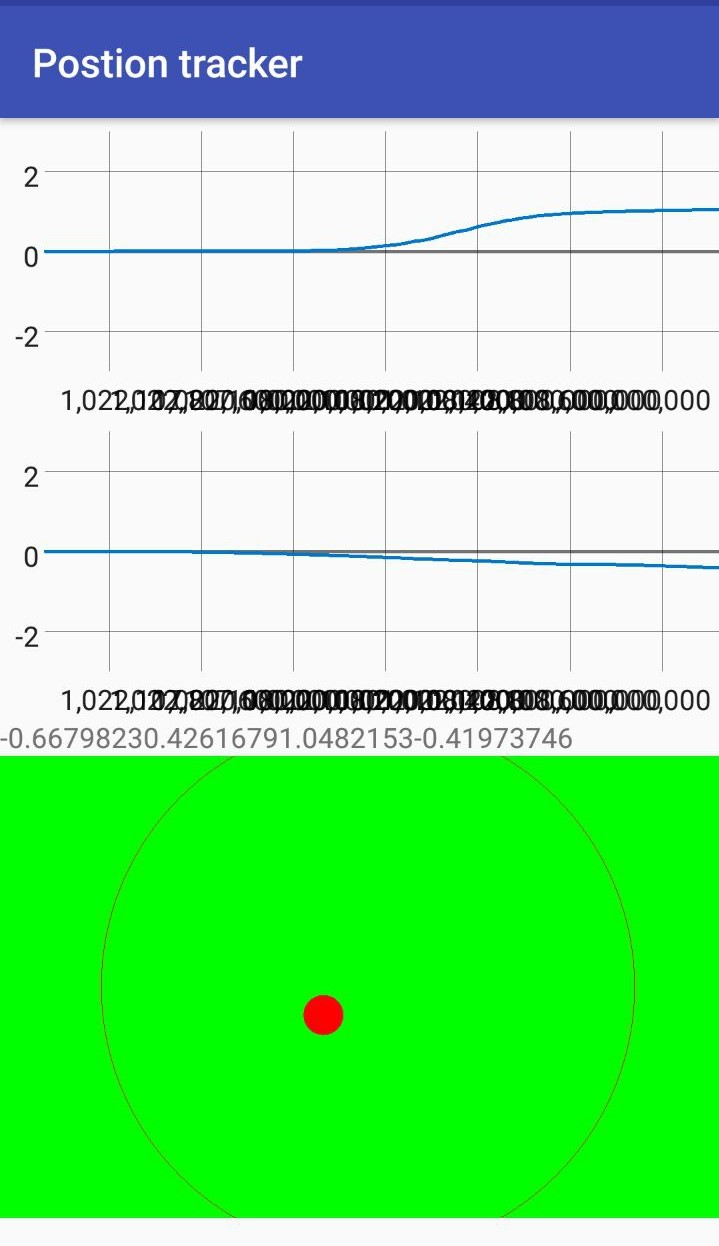
\includegraphics[width=0.5\textwidth]{figures/app1}
		\caption{Image of the position tracker app after conducting the test}
		\label{fig:app1}
	\end{center}
\end{figure}

\section{Discussion}
\label{sec:discussion}
xxxxx xxxx xxxx 

\bibliography{II2202-report}
%%\bibliographystyle{IEEEtran}
\bibliographystyle{myIEEEtran}
\appendix
\section{Insensible Approximation}

Note that the Appendix or Appendices are Optional.


\end{document}
